%% Technical-Analysis.tex
%% Mac Radigan
\documentclass{report}
\usepackage{graphicx,amssymb,amstext,amsmath,amsthm,caption,hyperref,mathtools}
\hypersetup{
 colorlinks,%
 citecolor=blue,%
 filecolor=blue,%
 linkcolor=blue,%
 urlcolor=blue
}
\newcommand\Quote[1]{\lq\textsl{#1}\rq}
\newcommand\fr[2]{{\textstyle\frac{#1}{#2}}}
\begin{document}
%-----------------------------------------------------------
\title{Technical Analysis Notes}
\author{Mac Radigan}
\date{} % comment this out if you would like to include the date
\maketitle
%-----------------------------------------------------------
\begin{abstract}\centering
This provides a general overview of techniques used for technical analysis.  Some general concepts of analysis are addressed, as well as particular techniques and formulae.  It also provides the framework and notation that will be utilized in analysis throughout the course.  Most importantly, it focuses on particular techniques that will be applied during trading, and further analyzed in furture reports.  For these particular techniques, examples are given of their application.  There is a discussion of their strengths, as well as why they were chosen.
\end{abstract}
%-----------------------------------------------------------
\tableofcontents
\listoffigures
%-----------------------------------------------------------
\chapter{Introduction}
 
\section{Context and motivation}\label{intro}
Using passed behavior as an indication of future behavior, through technical analysis one may utilize observed patterns within the market as a means of improving a portfolio's performance.  If the rate and probability of a stock's change in price can be characterized, and modelled, it can be used as a factor in trading decisions.  When a stock's performance closely follows the trader's model, significant gains may be realized.  Likewise, significant deviations of the stock's behavior from the model may result in losses when applying technical analysis to a portfolio.

\section{Notation Used}
When analyzing stocks, a set of fundamental signals is typically considered.  Each discrete data point in the signals is the aggregate decimation factor (period) of the underlying higher fidelity signal.  The components of this set are typically as follows:  date/time, open, close, high, and low.  The most often quoted period is a single day, but the period under consideration may be as granular as minutes for day traders or as course as months or years for long-term investors.  The notation used herein (and throughout future reports for this class) is given by Eq.~\eqref{eq:notationSet}.
%
\begin{flalign}
\label{eq:notationSet}
\mathcal{S}_{\ell,n}&=\{d_{\ell,n},o_{\ell,n},c_{\ell,n},h_{\ell,n},l_{\ell,n}\} \\
{} & \mbox{where} \nonumber \\
{} & d_{\ell,n} \mbox{ is the date/time signal with sample period $\ell$ } \nonumber \\
{} & o_{\ell,n} \mbox{ is the first value of each period ($\ell$) of the price signal} \nonumber \\
{} & c_{\ell,n} \mbox{ is the last value of each period ($\ell$) of the price signal} \nonumber \\
{} & h_{\ell,n} \mbox{ is the maximum value over each period ($\ell$) of the price signal} \nonumber \\
{} & l_{\ell,n} \mbox{ is the minimum value over each period ($\ell$) of the price signal} \nonumber 
\end{flalign}
\captionof{figure}{Stock Signal Notation}
\par
When no period is mentioned, we assume the period is equal to a single trading day.  Note that the actual date time is parameterized by the index $n$, allowing us to write equations using this discrete ordinal.  The value $n$ can later be cross-referenced using the signal $d$ to obtain the actual time that the sample was taken.  This distinction becomes particularly important in calculations that involve rates of change with respect to time.  While the market remains closed over the weekend, the discrete date/time signal $d_{n}$ does not contain those samples, whereas the continuous time variable $t$ does.  Thus, there is a periodic time compression of the above signals.  It would be possible to develop a system that includes days in which the mareket is closed by interpolating over this interval.  However, this in not starndard practice in modern trading systems.
\par
All of the signals in the set $\mathcal{S}$ can be derived from the underlying price signal, $P$, as shown in Eq.~\eqref{eq:notationOpen}-Eq.~\eqref{eq:notationLow}.  Note that samples from the derived signal correspond to the end of each period under consideration.
%
\begin{flalign}
\label{eq:notationOpen}
o_{\ell,n}&=p_{n-\ell} \\
{} & \mbox{where } \ell \mbox{ is the period under consideration} \nonumber
\end{flalign}
\captionof{figure}{Opening Price}
%
\begin{flalign}
\label{eq:notationClose}
c_{\ell,n}&=p_{n}
\end{flalign}
\captionof{figure}{Closing Price}
%
\begin{flalign}
\label{eq:notationHigh}
h_{\ell,n}&=\{p_{i} \geq p_{j} | p_{i},p_{j} \in P \mbox{ and } i,j \in [n-\ell, n] \} \\
{} & \mbox{where } \ell \mbox{ is the period under consideration} \nonumber
\end{flalign}
\captionof{figure}{High Price}
%
\begin{flalign}
\label{eq:notationLow}
l_{\ell,n}&=\{p_{i} \leq p_{j} | p_{i},p_{j} \in P \mbox{ and } i,j \in [n-\ell, n] \} \\
{} & \mbox{where }\ell \mbox{ is the period under consideration} \nonumber
\end{flalign}
\captionof{figure}{Low Price}
%
\par
Definitions presented herein will make use of this fundamental notation.  For generality, most of the equations presented will refer to a generic signal $X$.  Unless otherwise noted, it is assumed that the closing price is used ($X=C$), and the period in question is one day ($\ell=\mbox{ 1 day}$).
%

\section{Concepts and Strategies}
%

\subsection{Simple Trends}
%
Using simple trending techniques one classifies a market as one of upwards, downwards, and sideways.  It is based on the assumption that when prices are increasing or decreasing (upwards or downwards), they will continue in a similar manner.  When prices have see no significant change over the interval under consideration the market is said to be sideways.
\par
When using any technical indicator, it is always important to take volume into the volumes of trades occurring during that period into account.  A high volume confirms the market sentiment of the current trading price.  Price changes accompanied by lower volume are considered less stable as there is a smaller market sharing the sentiment \cite{Wealth}.


\subsection{Broader Market Trends}
%
When analyzing the performance of a particular stock, it is important to keep it in context of the broader market.  Trends seen by indexes such as the Dow Jones Industrial Average (DJI), may be a good indicator that the the market forces will also have an effect on the stock under consideration.  The indexes comprised of stocks within the same sector as that under consideration can also be used as a trending indicator \cite{Bonon}.
%
\subsection{Channels}
%
To help visualize a simple trend, investors will consider the local maxima of the hich price and the local minima of the low price of a stock, in an effort to determine a trend that predicts what the maximum and minimum price at which a stock trade will trade in the market \cite{Barbara}.
%
\subsubsection{Pivots}
%
These extrema become significant indicators when they are accompanied by a reversal in the signal, called a pivot.  Pivots at a maximum are known as pivot highs Eq.\eqref{eq:pivotHigh}, whereas pivots at a minumum are known as pivot lows Eq.~\eqref{eq:pivotLow} \cite{Barbara}.
%
\begin{flalign}
\label{eq:pivotHigh}
Ph_{n}^{M}&=\begin{cases}1, & h_{i}<h_{i-1} \forall i \in [n-M,n] \mbox{ and } h_{j}>x_{j+1} \forall j \in [n,n+M]\\0, & \mbox{otherwise}\end{cases} \\
{} & \mbox{where } M \mbox{ is the order of the pivot } \nonumber 
\end{flalign}
\captionof{figure}{Pivot High}
%
\begin{flalign}
\label{eq:pivotLow}
Pl_{n}^{M}&=\begin{cases}1, & l_{i}>h_{i-1} \forall i \in [n-M,n] \mbox{ and } l_{j}<l_{j+1} \forall j \in [n,n+M]\\0, & \mbox{otherwise}\end{cases} \\
{} & \mbox{where } M \mbox{ is the order of the pivot } \nonumber 
\end{flalign}
\captionof{figure}{Pivot Low}
%
Multiple pivots within a short interval are referred to as a multiple tops Eq.~\eqref{eq:multipleTop} and multiple bottoms \cite{Barbara}.
%
\begin{flalign}
\label{eq:multipleTop}
MultipleTop_{n}^{M}=\begin{cases}
  1, & \sum\limits_{k=n-\ell}^{\ell}Ph_{ n=h_{Ph_{n}} }>M \\
  0, & \mbox{otherwise}
\end{cases} \\
{} & \mbox{where } M \mbox{ is the multiplicity of the multiple top} \nonumber 
\end{flalign}
\captionof{figure}{Multiple Top}
%
\begin{flalign}
MultipleBottom_{n}^{M}=\begin{cases}
  1, & \sum\limits_{k=n-\ell}^{\ell}Pl_{ n=l_{Pl_{n}} }>M \\
  0, & \mbox{otherwise}
\end{cases} \\
{} & \mbox{where } M \mbox{ is the multiplicity of the multiple bottom} \nonumber 
\end{flalign}
\captionof{figure}{Multiple Bottom}
%
\subsection{Support/Resistance}
%
Trending of the minimum and maximum price asked by the market is often performed.  
%
By connecting adjoining pivot lows, a line can be drawn known as the support.  Support shows the very minimal price that the market is willing to sell over an interval, and can be extrapolated into the future performance of a stock as a lower limit that the price should not be expected to exceed.  
\par
By connecting adjacent pivot highs, a line can be drawn known as the resistance.  Resistance shows the maximal price that the market is willing to pay over an interval, and can be extrapolated into the future performance of a stock as the upper limit that the price should not be expected to exceed.
\par
The area between the support and resistance line is known as the channel.  When a price leaves the boundaries of the channel, it is said to have broken support/resistance. The higher the order of the pivots that comprise the support and resistance lines, the less likely the the price will break support/resistance (as historical evidence would show).  The contribution of multiple-top/bottom signals even further reduces the likelihood of a break from the channel.  With even greater certainty, the strongest line of support is given by the 52-week low $(l_{52 wk,n})$,  and the strongest line of resistance is given by the 52-week high $(h_{52 wk, n})$ \cite{Wealth}.
\par
Lines of support are chosen over intervals of the pivot low signal, using the extreme and second most extreme elements withing the interval.  These lines of support and resistence are considered valid only if the corresponding pivots within the given interval deviate from their least squares regression by a specified mean square error (MSE).
\par
When downsampling the pivot signals, care must be taken not to use decimation.  As the support and resistance lines developed from the first and second most maximal/minimal elements in the signal, those samples should also be preserved in the downsampled signal.
\par
%
\subsubsection{Example - Channels}
%
Consider LMT in 2009, with a trading range of \$57.50 and \$65.80 per share.  In the Fig.~\ref{fig:channels}, Pivots of order one are shown in green $(P_{n}^{1})$, and pivots of order two are shown in blue $(P_{n}^{2})$.  The pivots have been connected to form the channel.  Upward trends are drawn in blue, downward trends in red. Between January and March, the stock had a high volatility, resulting in a wide channel.  The channel narrows betweeen March and May, when the volatility of the stock has lowered.
%
\begin{figure}[ht]\centering
\label{fig:channels}
\includegraphics[width=1\textwidth]{figures/Channels-LMT-1.eps}
\caption{$\mbox{Channels and Pivot Points } LMT \approx 2009$}
\end{figure}
%
\subsubsection{Triangles}
%
If a has a dramatic decrease in volatility over a short period of time, channel narrows as the support and resistance lines close together.  As the lines approach a point of intersection, the stock is expected to have a sudden dramatic increase in volatility, then continue to rise or fall in its given direction.  This sudden change is known as a breakout \cite{Barbara}.  The pattern described by the support/resistance lines prior to this occurance are known as a triangles, pennants, and wedges because of their familiar shape.
%
\begin{figure}[ht]\centering
\label{fig:triangles}
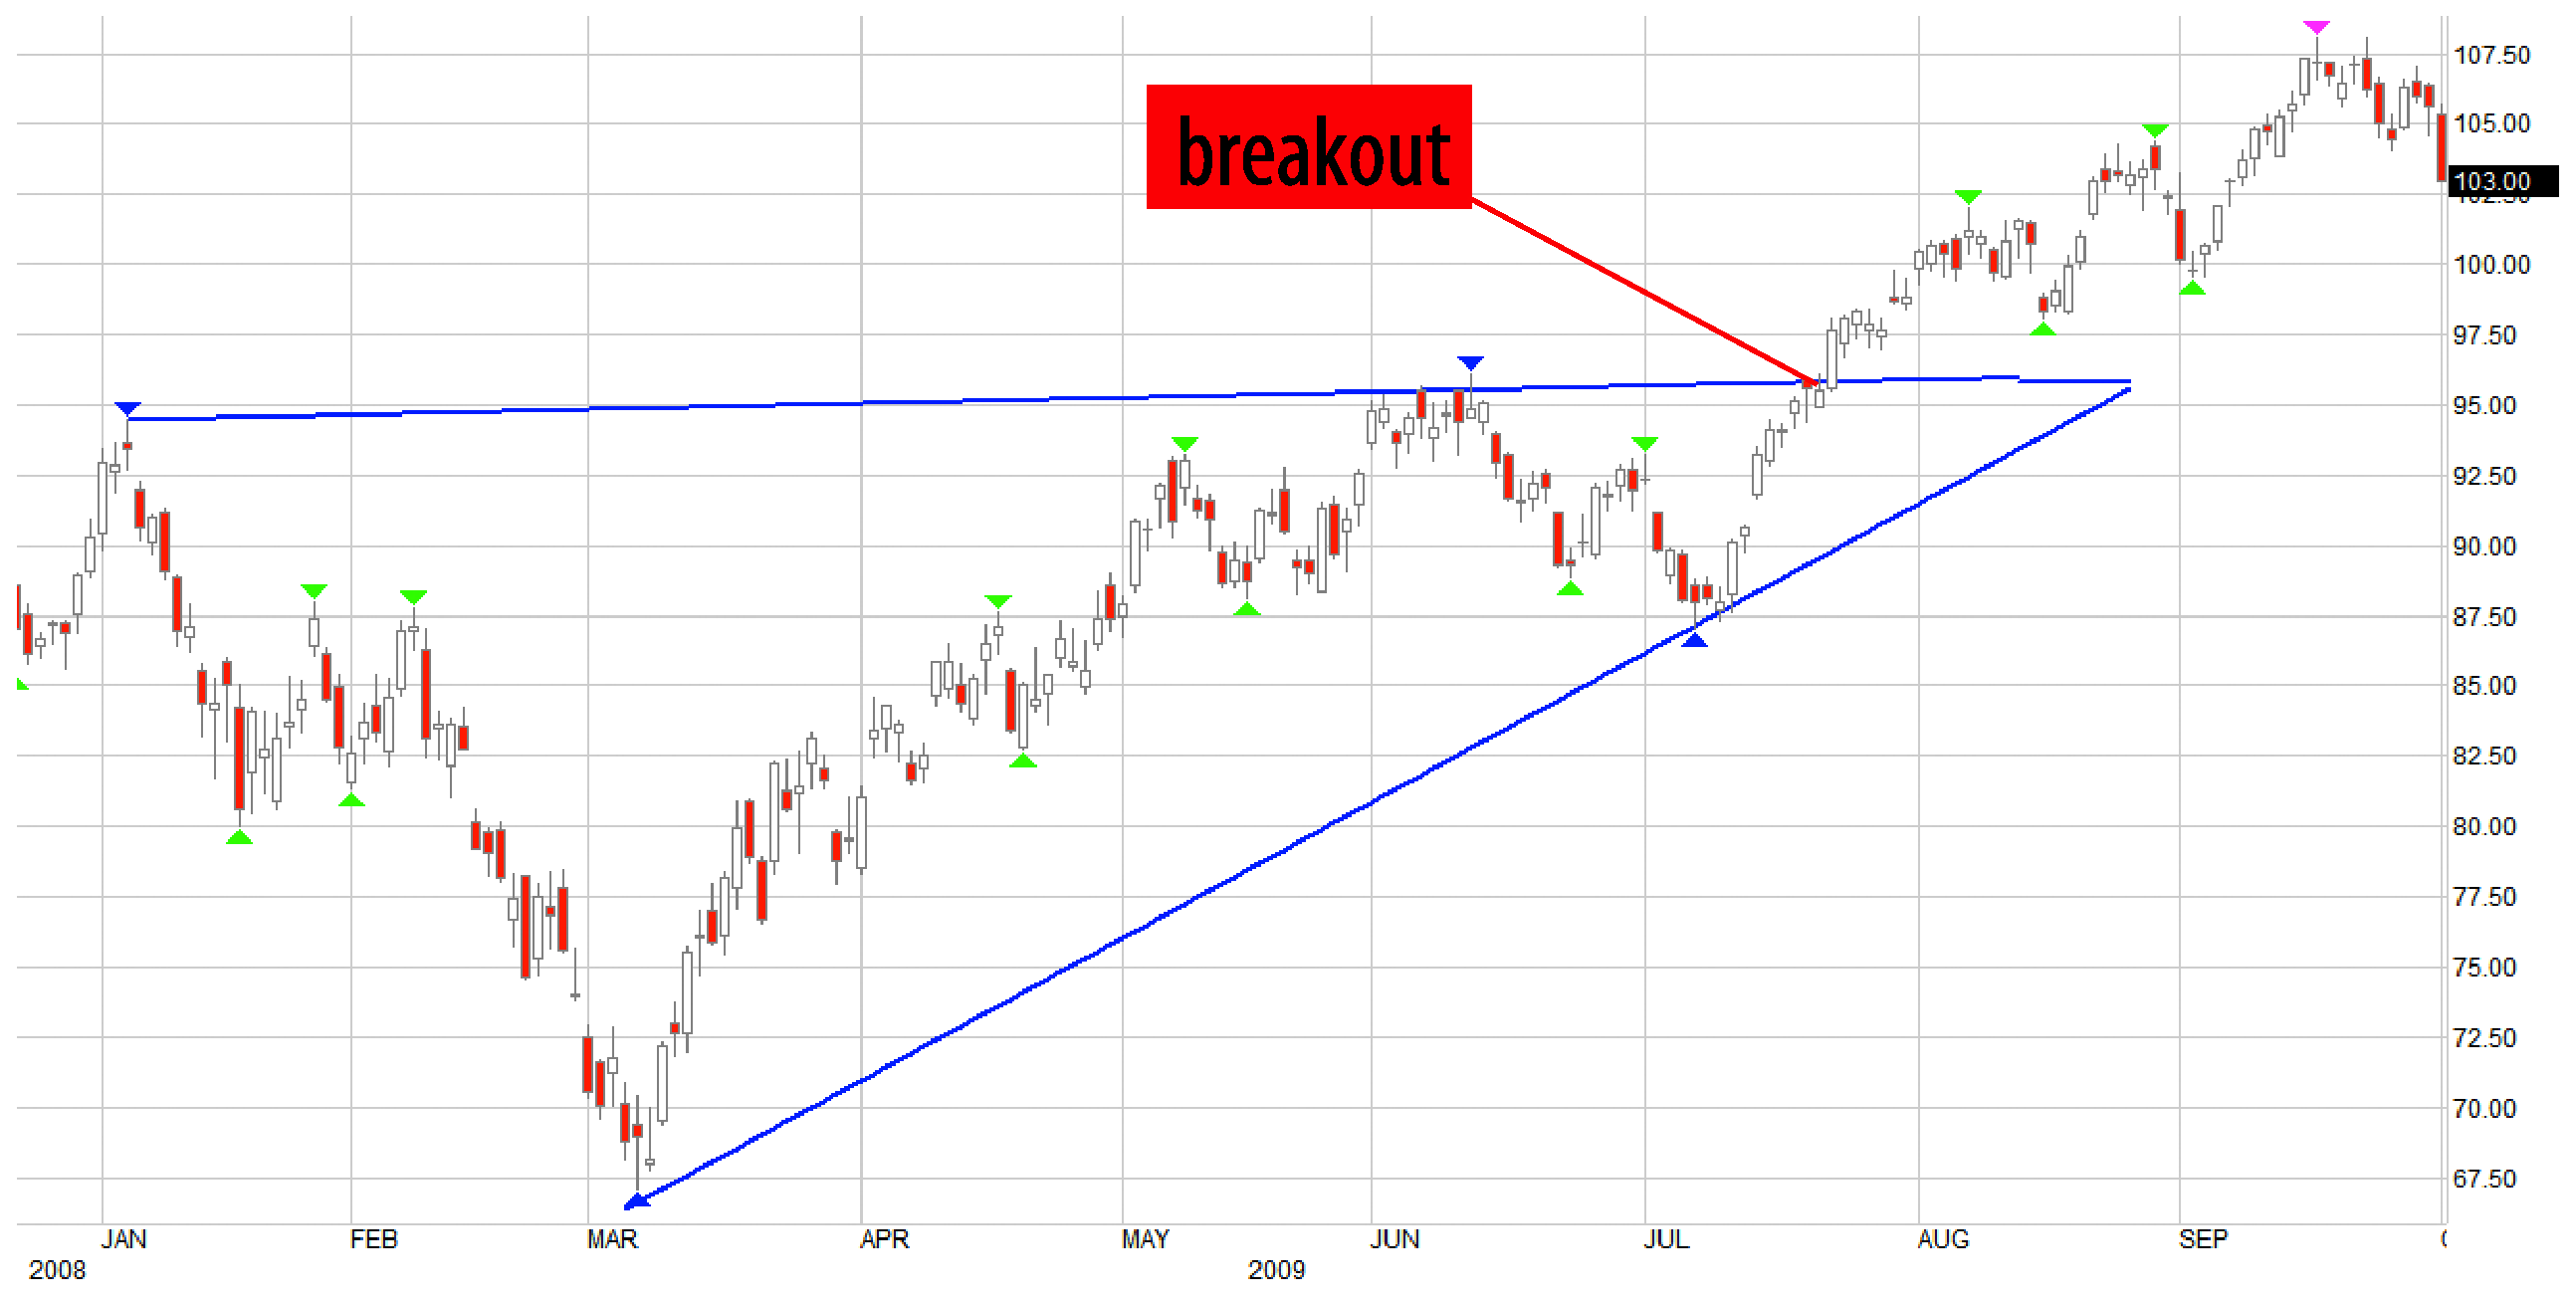
\includegraphics[width=1\textwidth]{figures/Triangle-SPY-1.eps}
\caption{$\mbox{Breakout from a Triangle} SPY \approx 2009$}
\end{figure}
%
\subsection{Accumulation/Distribution}
%
The price of a stock stocks generally show a cyclic behavior, oscillating between a bull and bear market.  During the beginning phase of a bull market, accumulation, the price of a particular stock is low, and considered to be underbought.  Investor interest builds momentum, driving the stock prices higher.  This is the beginning phase of the bear market, distribution, in which the stock price is beginning to reach a point where it is considered to be bought, driving prices down\cite{Bonon}.
\par
One important technique used in technical analysis is being able to predict when a stock is overbought or oversold, before the price signals change direction.  These inflection points in the price signals are known as reversals.  Often, predictive systems are used in technical analysis which attempt to report the current price as a percentage of the accumulation and distribution cycle.  Such measures are known as oscillators \cite{Barbara}.
%
\subsection{Retracement}
%Retracement/Correction/Pullback/Throwback
%
As prices rise (or fall) in a trend, there is a tendency for the price to take a corrective action in the opposite direction (called a retracement), as investors consider that the price may have reached an extreme, triggering an acion to sell (or buy).  After this short-term movement, the stock price then again continues in the direction of the overall trend \cite{Barbara}.  
\par
When purchasing a stock, it is not optimal to pay the highest price the market is willing to ask.  Waiting for the retracement allows investors to purchase a rising stock, at the price it will likely be at a short-term low.
%
\subsubsection{Bullish Retracement}
\label{bullishRetracement}
%
Short-term investors may make use of the retracement in a technique called a bullish retracement.  In this technique the investor wishes to enter a position to take advantage of a bullish trend.  Waiting until a retracement occurs, the stock is purchased at a locally low price.  The stock then again rises with the overall trend, and the investor holds the stock until such time as deemed favorable, when the price has risen above both the retracement price, as well as the original price prior to the retracement.   In this manner, the investor realizes gains since the original stock price, plus the gains from the difference of the original price and the retracement price \cite{Wealth}
\par
A bullish retracement is typically executed as a stop-limit order.  To help ensure the trade is entered during an upward price movement, a stop may be set at a \%ATR above the current price (see Sec.~\ref{ATR}).  Additionally, a limit may be set at some \%ATR below the current price as a way to automatically exit the position if the assumption about the direction of the movement turns out to be incorrect.

%
\subsubsection{Example - Bullish Retracement}
%
Consider ARMH on 20-Oct09 trading around \$7.83 per share.  At this time the ARMH is in a strong upward trend.  The subsequent day, the stock enters into retracement, and continues its downward path until reaching support on 28-Oct-09 at the price of \$7.00 per share.  At this time the stock has an ATR of \$0.23 per share.  If an investor places a stop order one ATR above the current price (\$7.23), the position will be entered when it leaps to \$7.26 on the subsequent day.  If the position is held until it reaches resistance, the sale will be made on 18-Nov-09 at the price of \$8.47 per share.
\begin{center}
\fbox{$(\frac{c_{18Nov}}{c_{28Oct}}-1) \times 100=(\frac{\$7.23}{\$8.47}-1) \times 100=17.15\%\mbox{ ROI}$}
\end{center}
%
\begin{figure}[ht]\centering
\label{fig:retracement}
\includegraphics[width=1\textwidth]{figures/Retracement-ARMH-1.eps}
\caption{$\mbox{Retracement} ARMH \approx 2009$}
\end{figure}




\chapter{Average Price}

\section{Overview}
Moving averages (MA) are smoothing filters which help to visualize a trend over a specified interval.  Each data point in the filtered signal is an averaging over the specified interval. These low pass filters (LPFs), eliminate noise in the price signal.  This indicator lags the input signal (price signal).
\par
If the filter is implemented digitally in the time domain, then increasing the number of samples in the filter interval has the effect of lowering the cutoff frequency of the LPF in the frequency domain, and thus decreasing the responsiveness to short term trends.  Contrariwise, decreasing the number of samples in the filter interval increases the cutoff frequency seen in the frequency domain, thus making the moving average more responsive to short term trends.
\par
Unless otherwise noted, references made herein to the moving average refer to the simple moving average (Sec.~\ref{price:SMA}), and depicted by overloading the common notation for averages $\bar{X}$.  Although sometimes useful to center the filter on the current sample (central moving average), for the methods discussed herein the filters are causal.
\par

\section{Simple Moving Average}\label{price:SMA}
The simple moving average (SMA) have the form Eq.~\eqref{eq:SMA}. They apply an equal weighting to each sample in the filter, ($\frac{1}{N}$), and tend to lag the input signal significantly.
%
\begin{equation}
\label{eq:SMA}
SMA_{N}\{x\}_{n}=\frac{1}{N}\sum\limits_{k=0}^{N}x_{n-k}
\end{equation}
\captionof{figure}{Simple Moving Average}
%
\par
%
\section{Exponential Moving Average}
Weighted moving averages (WMA) apply a different weighting coefficient to each sample in the average, whereby emphasizing and de-emphasizing particular samples.  By applying heavier weights to more recent samples, the lag of the filter can be reduced, resulting in an indicator that more closely matches the current trend.  
\par
In all weighted averages, the result is normalized such that the sum of the weights in the filter add up to the number of filter samples.  That is, the following condition must hold for all weights $w_{i}$ in the filter:
\begin{equation}
\label{eq:averageNormalization}
\sum\limits_{i=1}^{N}w_{i}=N
\end{equation}
\captionof{figure}{Normalization Condition for Moving Averages}
\par
In the case of the exponential moving average (EMA), an exponentially decreasing weight is applied to each successive sample in reverse time ($w_{i}=\frac{1}{(1-\alpha)^{i}}$).  The average is normalized as described above Eq.~\eqref{eq:averageNormalization}.
\begin{equation}
EMA_{\alpha,N}\{x\}_{n}=\frac{\sum\limits_{k=0}^{N}(1-\alpha)^{k}\cdot x_{n-k}}{\sum\limits_{k=0}^{n-k}(1-\alpha)^{k}}
\end{equation}
\captionof{figure}{Exponential Moving Average}

\subsection{Example Application - Moving Average as an Indicator of a Trend}
Moving averages can be used as an indicator of trending over a specified period ($N$).  The first derivative of the moving average with respect to time gives an estimate of the rate of change ($v_{n}=\frac{\partial x}{\partial t}x_{n}$).  Likewise, the second derivative estimates the acceleration of the change in price ($a_{n}=\frac{\partial^2 x}{\partial t^2}x_{n}$).  The digital implementation leaves a variety of choices in differentiation filters to arrive at these derivatives.
\par
In Fig~\ref{MA} and LMT in 2009 can be seen along with a 10-day moving average of the closing price.
%%There is variety of choice in the digital implentation of the derivatives.  For the purpose of this example, the simple difference equations may be used Eq.~\eqref{eq:priceDerivatives}.
%%
%%\begin{flalign}
%%\label{eq:priceDerivatives}
%%v_{n} = p_{n}-p_{n-1} \\
%%a_{n} = v_{n}-v_{n-1} \nonumber
%%\end{flalign}
%%\captionof{figure}{Time Derivatives of Price}
\begin{figure}[ht]\centering
\label{MA}
\includegraphics[width=1\textwidth]{figures/EMA-10-LMT-1.eps}
\caption{$EMA_{N=10}\{c_{LMT \approx 2009}\}$}
\end{figure}

\section{Moving Average Convergence-Divergence (MACD)}
\label{MACD}
The Moving Average Convergence Divergence (MACD) is an indicator of the rate of change in stock price (an estimation of $v_{n}=\frac{\partial x}{\partial t}x_{n}$) \cite{Wikipedia:MACD}.
The indicator achieves this by computing a difference in EMAs with periods to two different lengths Eq.~\eqref{eq:MACD}.  As the average price of the shorter and longer trend estimations approach (convergence), the measure of the MACD approaches zero.  As the trends separate (divergence), the magnitude of the MACD increases.
%
\begin{flalign}
\label{eq:MACD}
MACD_{\alpha,N_{1},N_{2}}\{x\}&=EMA_{\alpha,N_{1}}\{x\}-EMA{\alpha,N_{2}}\{x\} \\
{} & \mbox{with typical values } N_{1}=12, N_{2}=24 \nonumber
\end{flalign}
\captionof{figure}{Moving Average Convergence-Divergence (MACD)}
\par
A function called the Signal (SIGNAL) Eq.~\eqref{eq:MACDSignal} is generally used as trigger for finding an inflection in the price signal.  It is a smoothing of the MACD signal, specifically an EMA of the MACD, with an EMA filter length slightly less than the short term trend component of the MACD itself.  When the MACD crosses up through the signal line (sometimes called a golden cross), an increase in price is predicted.  When the signal line crosses down through the MACD (sometimes called a dead cross), a decrease in price is predicted.  Thus, inflection points in the price are expected when the condition $MACD-Signal=0$ is met.  The Signal line crossing is found more reliable than the MACD zero crossing \cite{Wikipedia:MACD}.
%
\begin{flalign}
\label{eq:MACDSignal}
SIGNAL_{\alpha,N_{S},N_{1},N_{2}}\{x\}&=EMA_{\alpha,N_{S}}\{MACD_{\alpha,N_{S},N_{1},N_{2}}\{x\}\} \\
{} & \mbox{with typical values } N_{1}=12, N_{2}=24, N_{S}=9 \nonumber
\end{flalign}
\captionof{figure}{MACD Signal Line}
\par
To assist graphical displays, it is common to display a third signal called a Histogram (HIST) Eq.~\eqref{eq:MACDHistogram}.  The Histogram is the difference of the MACD and the Signal line, and is used for the sole purpose of displaying the histogram signal crossings.  For this purpose, it is usually plotted as a histogram, to emphasize the zero crossings without cluttering the other signals in the display.  Values of zero in the Histogram will predict inflections in the price signal \cite{Wikipedia:MACD}.
%Being the difference of the rate of change in price, the Histogram represents the acceleration of the price signal (a simple estimation of the true price acceleration $a_{n}=\frac{\partial^2 x}{\partial t^2}x_{n}$).  Values of zero in the Histogram will predict inflections in the price signal \cite{Wikipedia:MACD}.
%
\begin{flalign}
\label{eq:MACDHistogram}
HISTOGRAM_{\alpha,N_{S},N_{1},N_{2}}\{x\}&=MACD_{\alpha,N_{1},N_{2}}\{x\}-SIGNAL_{\alpha,N_{S},N_{1},N_{2}}\{x\} \\
{} & \mbox{with typical values } N_{1}=12, N_{2}=24, N_{S}=9 \nonumber
\end{flalign}
\captionof{figure}{MACD Histogram}

\subsection{Example - MACD as an Indicator to Buy/Sell}
As an example, consider LMT on 12-Mar-09 trading at \$60.97 per share.  On this day, the Histogram is zero, and the MACD crosses up through the Signal line (indicating prices will increase).  Using the MACD as the sole indicator, the trade is entered on this day.  
\par
The position is held until 03-Apr-09, when the Histogram is again zero.  An anxious investor may wish to sell at this time, at the share price of \$67.34 per share.  This lags the nearest previous local maximum of one day prior, 02-Apr-09 at a price of \$
69.24 per share.
\par
\begin{center}
\fbox{$(\frac{c_{03Apr}}{c_{12Mar}}-1) \times 100=(\frac{\$67.34}{\$60.97}-1) \times 100=10.44\%\mbox{ ROI}$}
\end{center}
At this time the MACD has not crossed under the Signal line, and on the next day (04-Apr-09), the MACD bounces back (increases relative to the Signal), with the next zero crossing not occuring unti 22-Apr-09, when the price of LMT was at \$74.97 per share.  The investor may exit the position at this time, as the following days the MACD oscillates through the Signal line, with indeterminant information.
\par
\begin{center}
\fbox{$(\frac{c_{22Arp}}{c_{12Mar}}-1) \times 100=(\frac{\$74.97}{\$60.97}-1) \times 100=22.96\%\mbox{ ROI}$}
\end{center}
If the investor awaits for the MACD to move a significant distance below the Signal, rather than tangential to it, the realization would occur on 07-May-09, at \$79.68 per share.
\par
\begin{center}
\fbox{$(\frac{c_{07May}}{c_{12Mar}}-1) \times 100=(\frac{\$79.68}{\$60.97}-1) \times 100=30.68\%\mbox{ ROI}$}
\end{center}
%
\begin{figure}[ht]\centering
\includegraphics[width=1\textwidth]{figures/MACD-factory-LMT-4-a.eps}
\caption{$MACD\{c_{LMT \approx 2009}\}$}
\end{figure}





\chapter{Measures of Momentum}
%

\section{Stochastic Oscillator}
%
The basis for the stochastic oscillator \eqref{eq:stochasticOscillator} stems from considerable historical evidence of prices closing near their high during upward trends, and prices closing near their low in downward trends.  The indicator is termed and oscillator because it fluctuates between two extrema.  The ratio is a percentage how close the current price is to the average high, relative to the range between the average high and low.
%
\begin{flalign}
\label{eq:stochasticOscillator}
\%K_{\ell,n} &= 100 \cdot (\frac{c_{n}-l_{\ell,n}}{h_{\ell,n}-l_{\ell,n}}) \\
{} & \mbox{where} \nonumber \\
{} & c_{\ell,n} \mbox{ is the closing price over the interval of $\ell$ } \nonumber \\
{} & h_{\ell,n} \mbox{ is the hight price over the interval of $\ell$ } \nonumber \\
{} & l_{\ell,n} \mbox{ is the low price over the interval of $\ell$ } \nonumber \\
{} & \mbox{with typical values $\ell$ = 14 days } \nonumber \\
\end{flalign}
\captionof{figure}{Stochastic Oscillator}
%
\par
A trigger line, given by equation \eqref{eq:stochasticOscillatorSignal} is used to determine when a price inflection will occur.  This trigger line is a three-period moving average of the stochastic oscillator.  It is estimated that an inflection will occur when these lines cross.
\par
%
\begin{flalign}
\label{eq:stochasticOscillatorSignal}
\%D = SMA_{N=3\ell}\{\%K\}
\end{flalign}
\captionof{figure}{Stochastic Oscillator Signal Line}
%
The figure below shows LMT in 2009 trading between \$57.11 and \$86.76 for the year.  The \%K and \%R lines for the stochastic oscillator are shown below, giving the same buy indicator during the upward trend 
%
\begin{figure}[ht]\centering
\label{fig:stochasticOscillator}
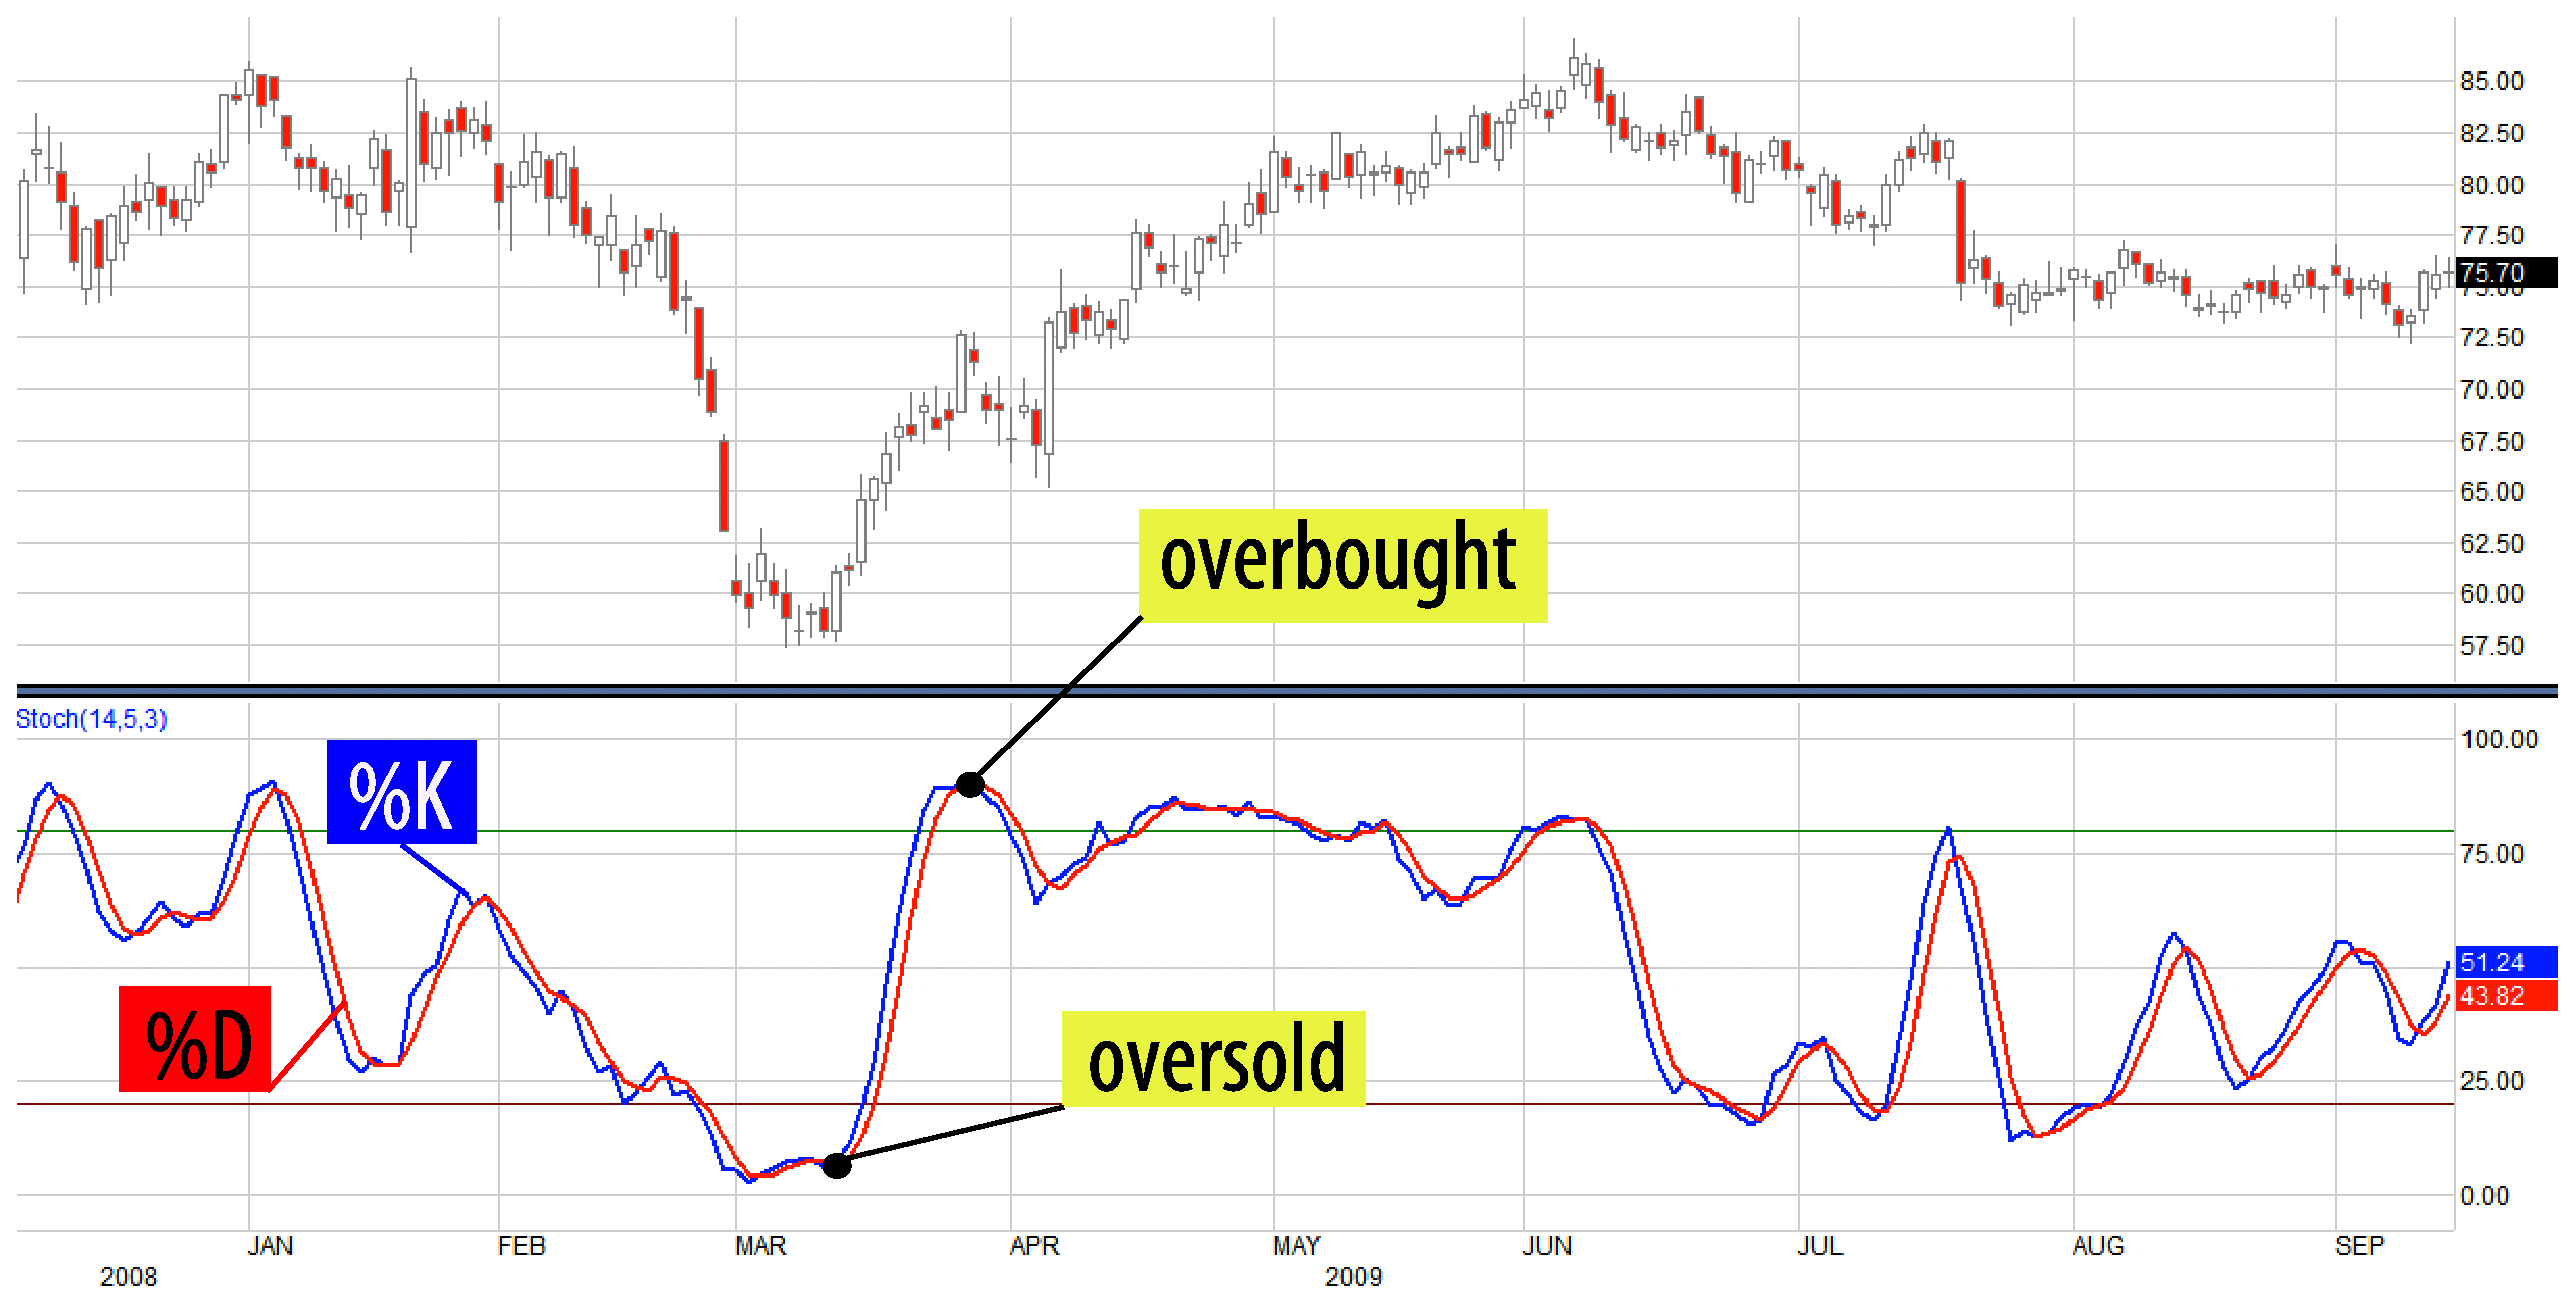
\includegraphics[width=1\textwidth]{figures/Stochastic-LMT-1.eps}
\caption{$\mbox{Stochastic Oscillator} LMT \approx 2009$}
\end{figure}
%
\subsection{Example Revisited - Comparison of Stochastic Oscillator to MACD}
%
Consider LMT around 12-Mar-09 as an example of the stochastic oscillator outperforming the MACD.  Although both indicators agree to enter the trade on this date, the stochastic oscillator triggers to sell at the local maxima on 03-Mar-09 at \$72.69 per share.  The MACD lags the signal, and triggers to sell on 03-Apr-09 at \$67.39 per share, for a differential of $-\$5.30$ per share.  This is illustrated in the figure below (Fig.~\ref{stochasticMACD}) with price signal (top chart), the stocastic oscillator (middle chart) and the MACD (bottom chart).
%
\begin{figure}[ht]\centering
\label{stochasticMACD}
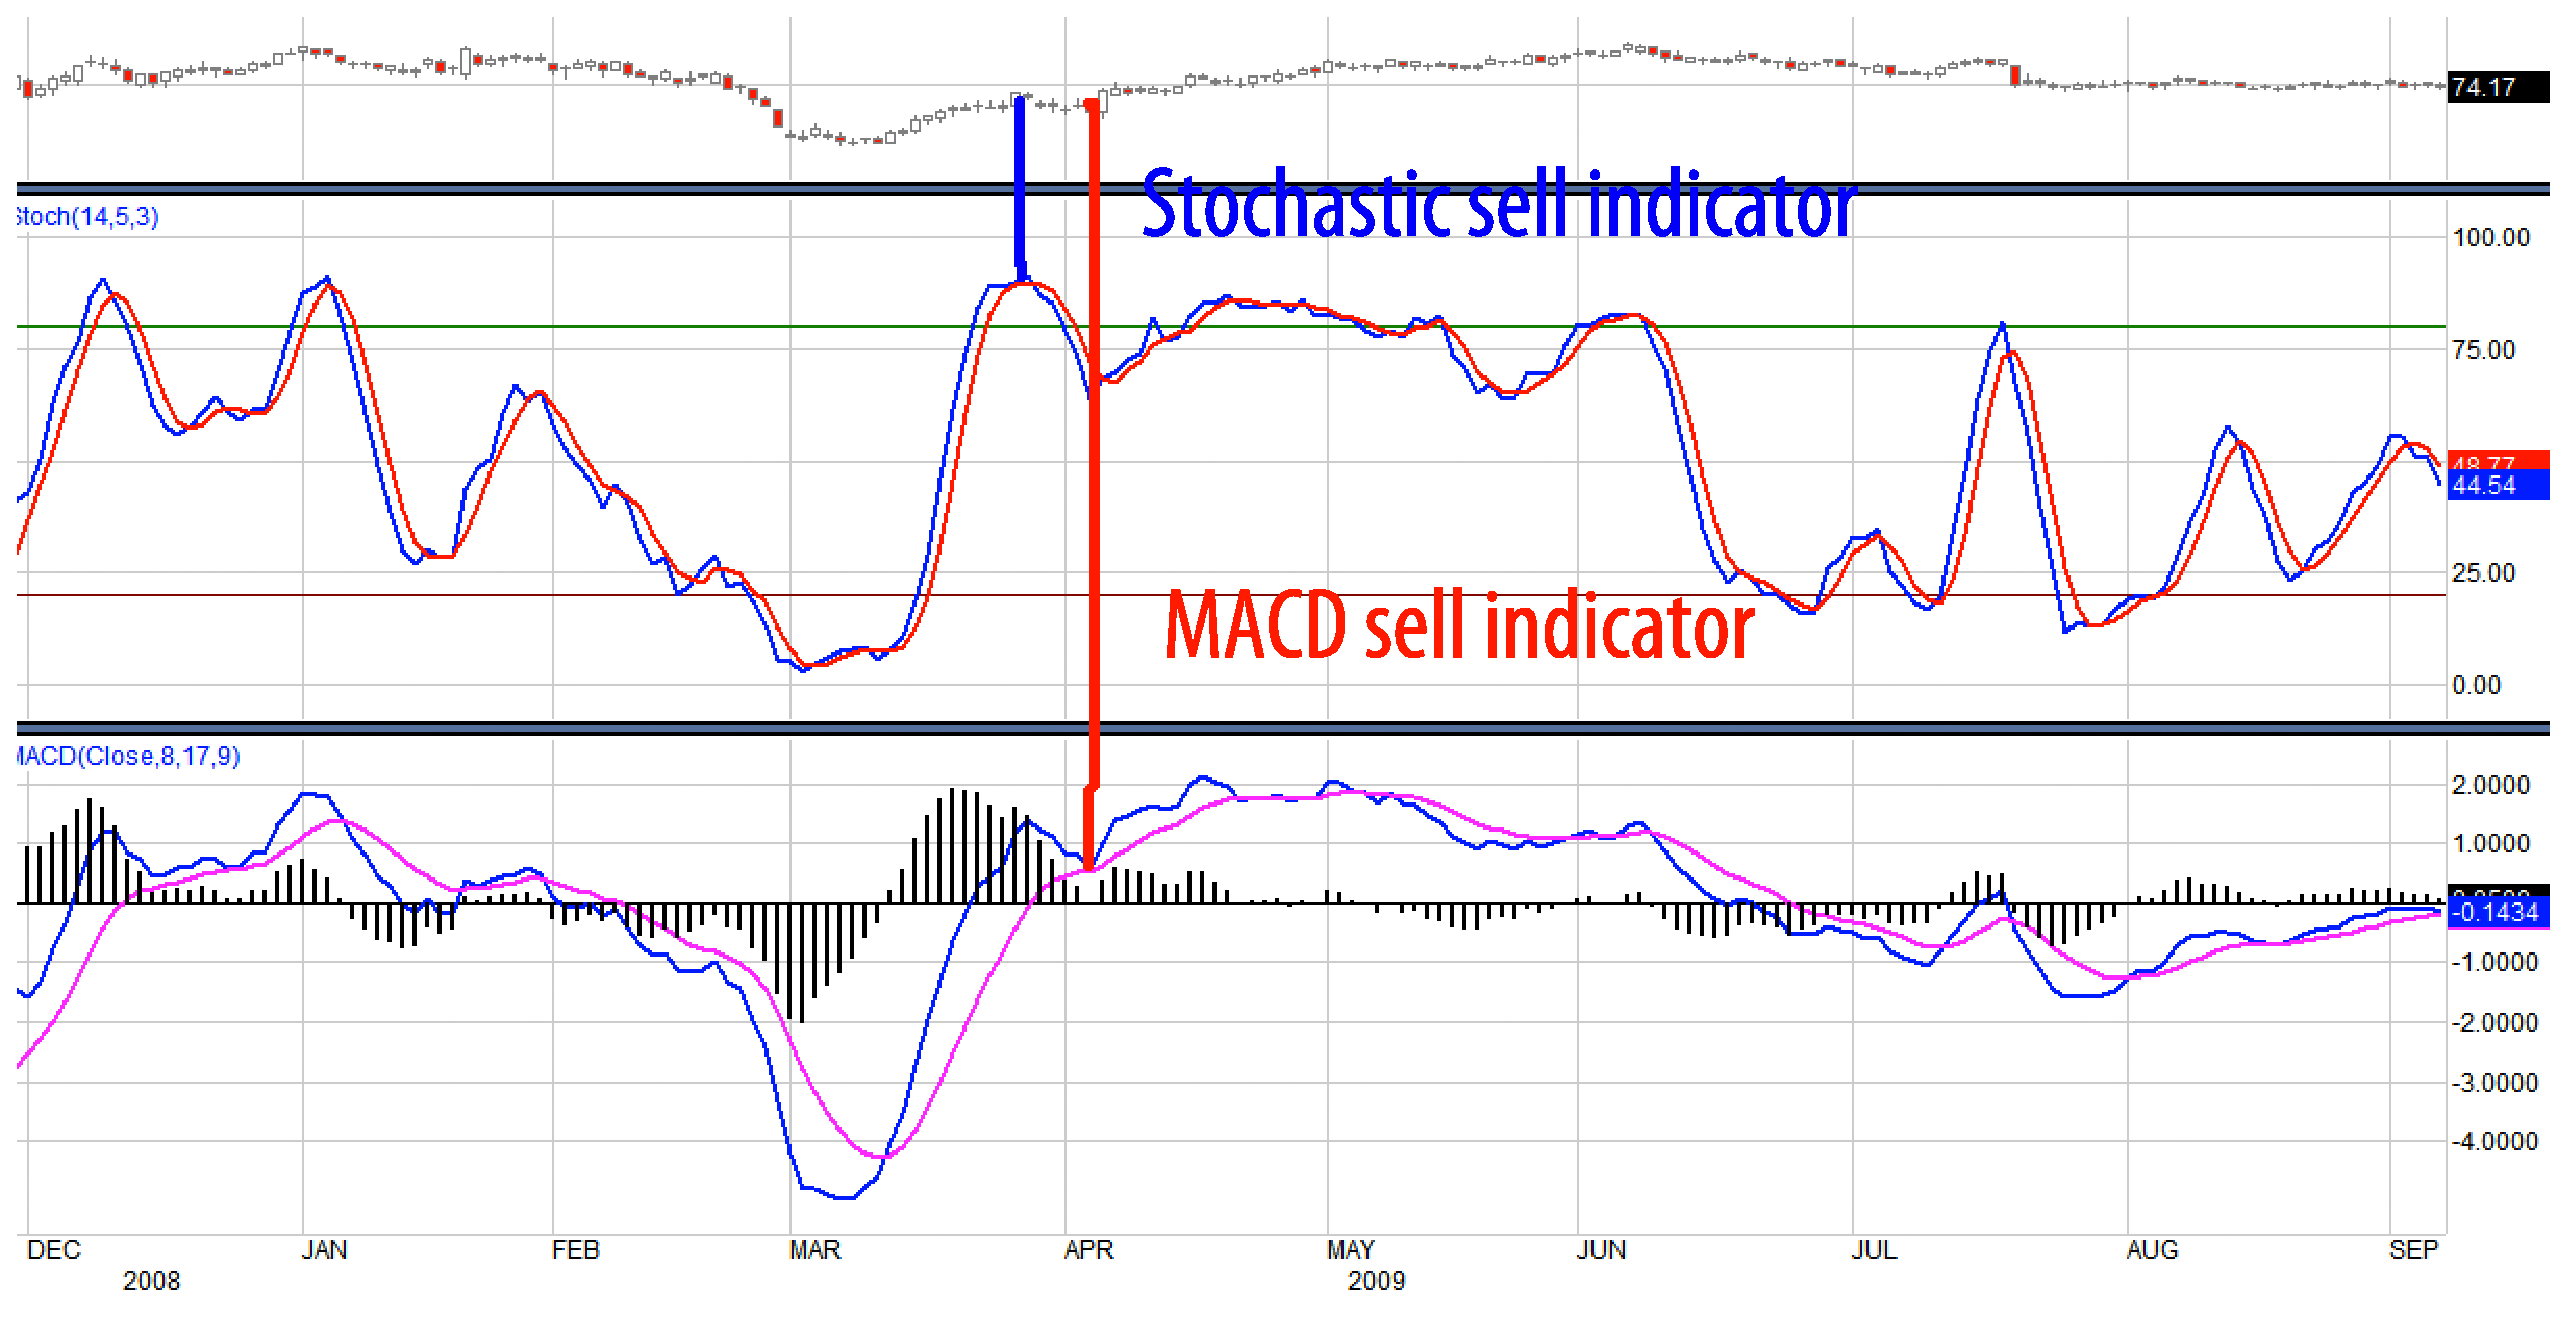
\includegraphics[width=1\textwidth]{figures/Stochastic-MACD-LMT-1.eps}
\caption{$MACD\{c_{LMT \approx 2009}\} \mbox{ and } \%K_{LMT \approx 2009}$}
\end{figure}
%
\section{Williams \%R}
%
The williams \%R \eqref{eq:williamsR} is similar to the stochastic oscillator, but is designed with a negative scale.  The oscillator stays in a range of $[0,-100]$.  When the williams \%R raises above -20 the stock is beleived to be overbought, and when the price drops below -80 it is beleived to be oversold \cite{Wikipedia:WilliamsR}.
%
\begin{flalign}
\label{eq:williamsR}
\%R_{\ell,n} &= 100 \cdot (\frac{c_{n}-h_{\ell,n}}{h_{\ell,n}-l_{\ell,n}}) \\
{} & \mbox{where} \nonumber \\
{} & c_{\ell,n} \mbox{ is the closing price over the interval of $\ell$ } \nonumber \\
{} & h_{\ell,n} \mbox{ is the hight price over the interval of $\ell$ } \nonumber \\
{} & l_{\ell,n} \mbox{ is the low price over the interval of $\ell$ } \nonumber \\
{} & \mbox{with typical values $\ell$ = 10 days } \nonumber \\
\end{flalign}
\captionof{figure}{Williams \%R}
%

\section{Chaikin Money Flow}
%
The Chaikin Money Flow (CMF) is an indicator based on the cumulative accumulation and distribution of a stock, thus taking volume into account.  Positive values reflect accumulation in the market, and negative values reflect distribution.  The extent and strenght of the accumulation/distibution is reflected by the duration (that it is positive/negative) and magnitude, respectively \cite{Investopedia:CMF}.
\par
To compute the CMF, the day's close of taken as a percentage of the range, known as the close location value (CLV) Eq.~\eqref{eq:CLV}.  This percentage is cumulatively added to the volume as a measure of the accumulationd/distribution Eq.~\eqref{eq:AD} \cite{Wikipedia:AccumulationDistribution}.
%
\begin{equation}
\label{eq:CLV}
CLV_{n}=\frac{(c_{n}-l_{n})-(h_{n}-c{n})}{h_{n}-l_{n}}
\end{equation}
\captionof{figure}{Close Location Value}
%
\begin{flalign}
\label{eq:AD}
AD_{n}&=AD_{n-1}+V_{n}CLV_{n} \\
{} & \mbox{where V is the volume in shares } \nonumber \\
\end{flalign}
\captionof{figure}{Accumulation/Distribution Index}
%
\begin{flalign}
\label{eq:CMF}
CMF_{n}&=EMA_{N_{1}}\{AD_{n}\}-EMA_{N_{2}\{AD_{n}\}} \\
{} & \mbox{with typical values $N_{1}=3$ and $N_{2}=10$ } \nonumber \\
\end{flalign}
\captionof{figure}{Chaikin Money Flow}
%
The Chaikin Money Flow is subject to failure during price breakouts and gaps, as the market deviates from the precedented buying and selling pressures \cite{Investopedia:CMF}.
%
\begin{figure}[ht]\centering
\label{CMF}
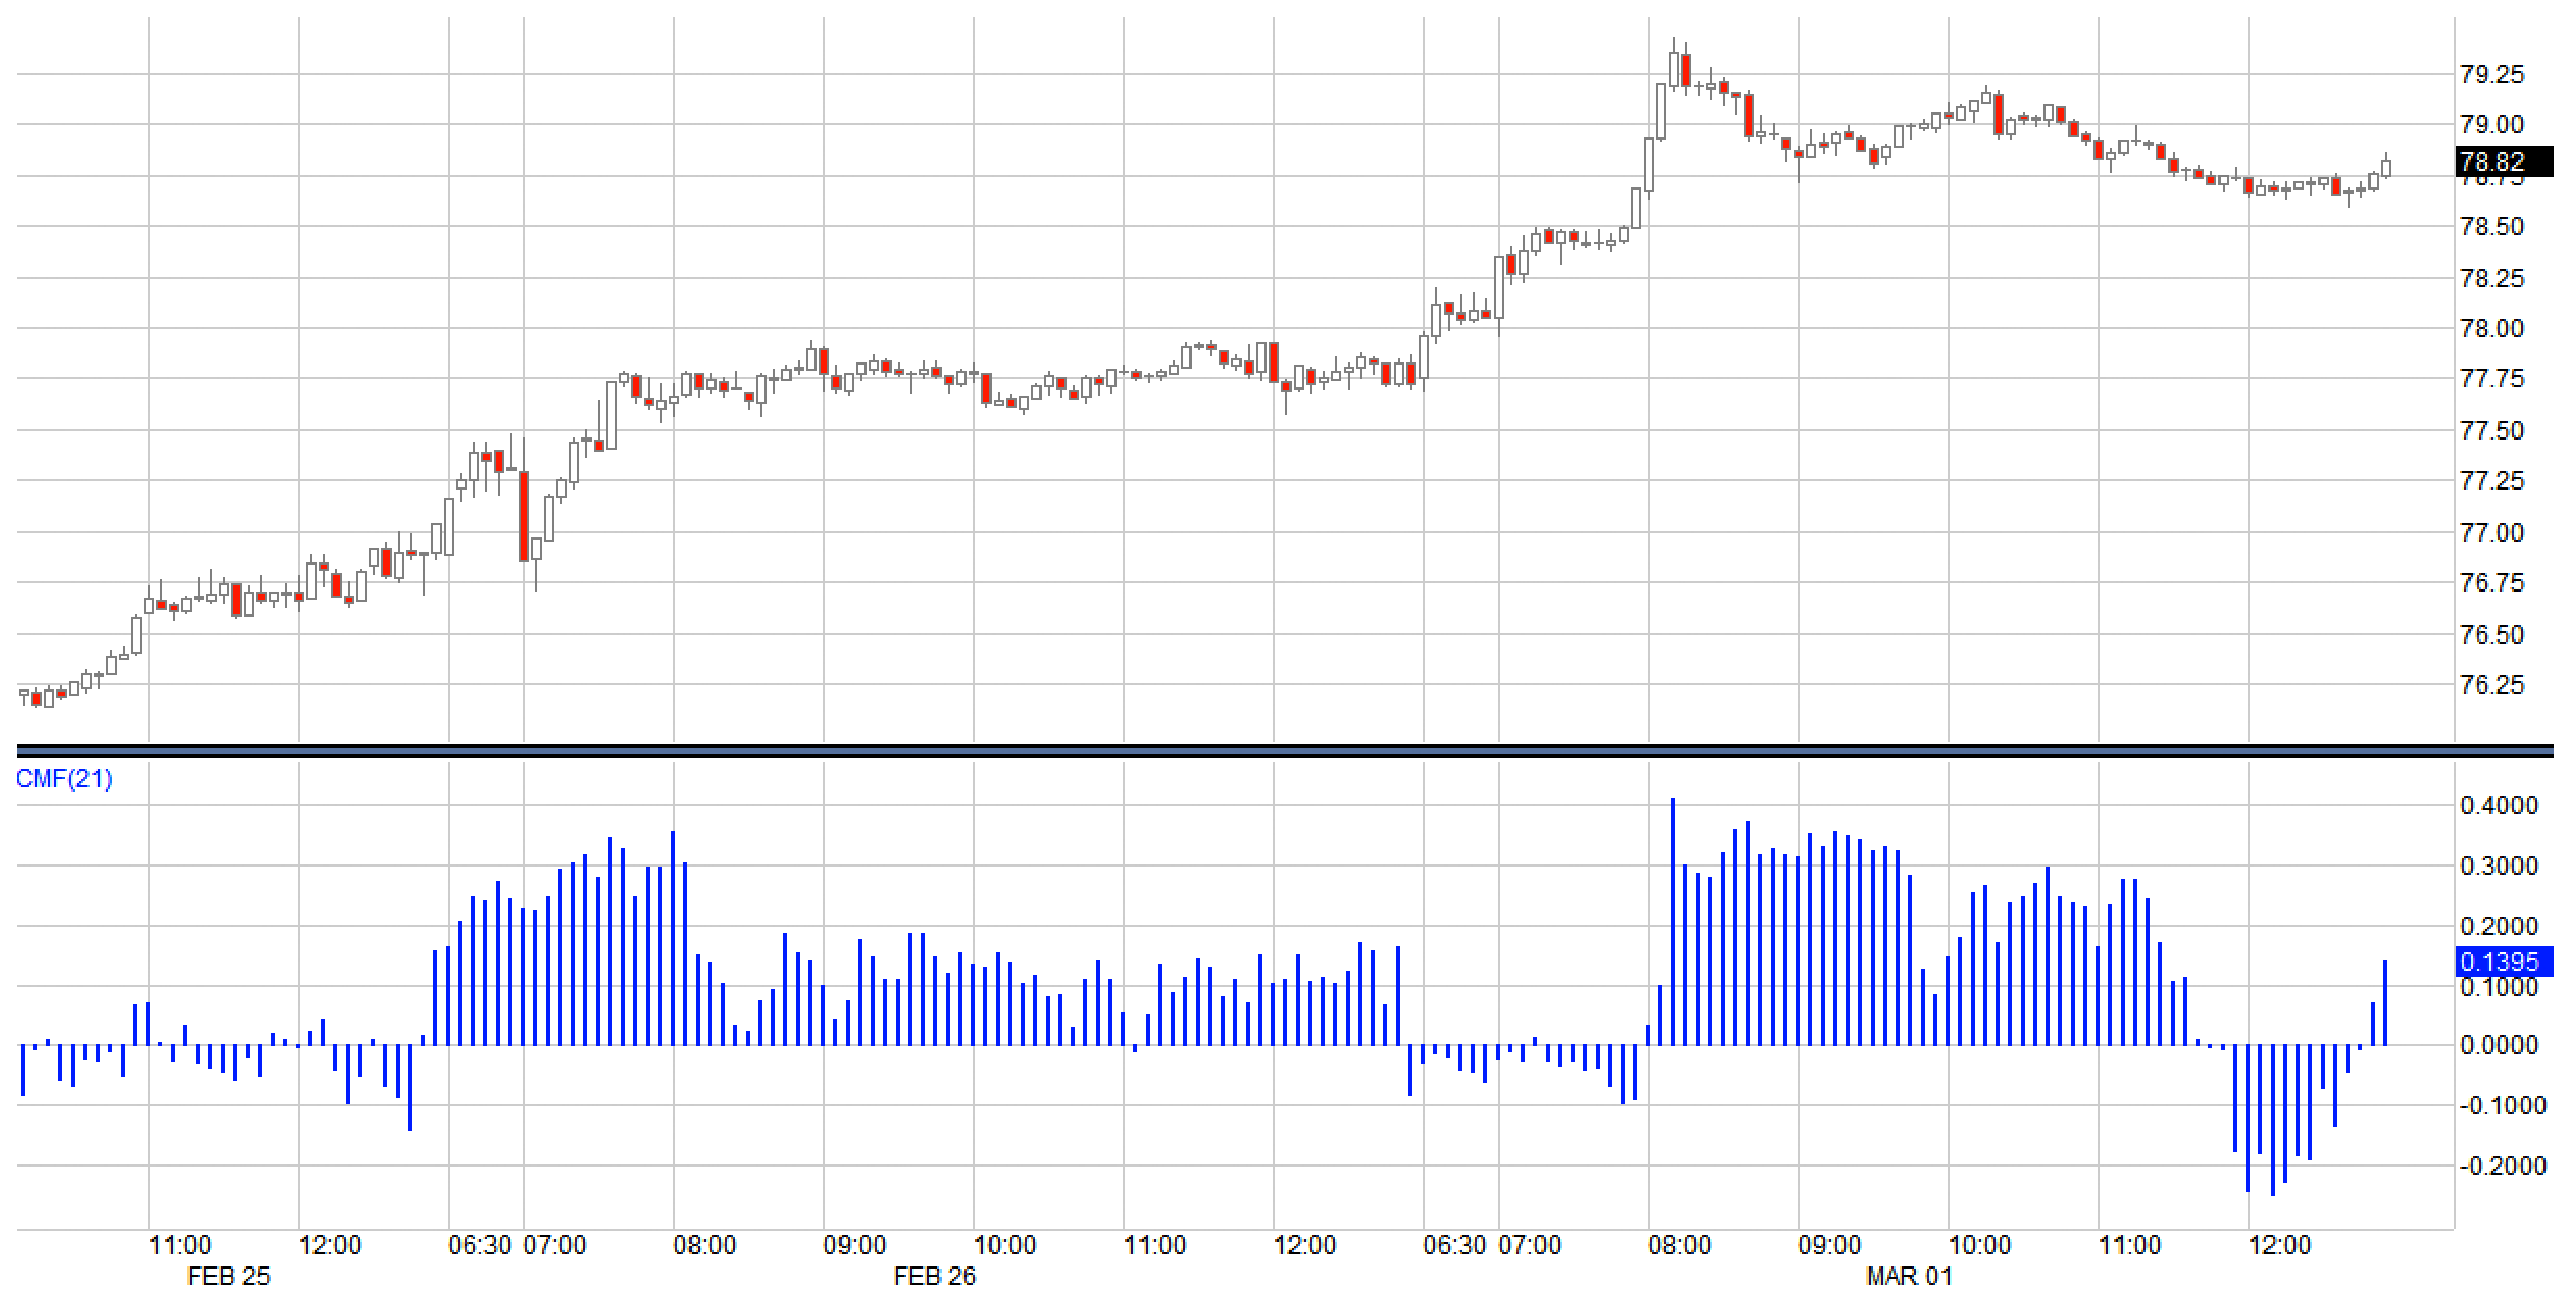
\includegraphics[width=1\textwidth]{figures/CMF-LMT-1.eps}
\caption{$CMF\{c_{LMT \approx 2009}\}$}
\end{figure}

%\section{Relative Strenght Index (RSI)}
%




\chapter{Measures of Volatility}
%
\section{Historical Volatility}
%
The historical volatility $(\sigma)$ of a stock Eq.~\eqref{eq:historicalVolatility} is the standard deviation of the stock price, usually taken over a 10-day period \cite{Dineen}.  As recent past performance of a stock may be a good indicator of recent future performance, it can be used as a benchmark in determining the risk of an investment, as well how far a stock price is likely to deviate from its moving average.  Some strategies, such as straddles (to be discussed later in the report on options), make use almost entirely on the volatility of a stock.
%
\begin{flalign}
\label{eq:historicalVolatility}
\sigma\{x\}_{n}&=\sqrt{\frac{1}{N}\cdot \sum\limits_{k=0}^{N}(x_{n-k}-SMA\{x\}_{n})^{2}} \\
{} & \mbox{with typical values } N=10 \nonumber
\end{flalign}
\captionof{figure}{Historical Volatility}
%
\section{Average True Range (ATR)}
\label{ATR}
%
The average true range (ATR) is an exponential moving average of the true range of a stock over a given period Eq.~\eqref{eq:ATR}.
%
\begin{equation}
\label{eq:ATR}
TR_{n}=\max(h_{n},c_{n})-min(l_{n},c_{n})
\end{equation}
\captionof{figure}{True Range}
%
\par
It is said that a stock is statistically unlikely to move more than one ATR in a given trading day.

%\section{Bollinger Bands}
%
%\section{On-Balance Volume (OBX)}
%
%\section{Volatility Index (IDX)}
%


%\chapter{Patterns}

\section{Gaps}
\begin{enumerate}
\item \textbf{Breakaway Gaps} - 
\item \textbf{Runaway Gaps} - 
\item \textbf{Exhaustion Gaps} - 
\item \textbf{Island Gaps} - 
\end{enumerate}

\section{Candle Stick Charting}
\begin{enumerate}
\item \textbf{Real Body} - 
\item \textbf{Shadow} - 
\end{enumerate}
%
\subsection{Doji}
\begin{enumerate}
\item \textbf{Plain Doji} - 
\item \textbf{Dragonfly Doji} - 
\item \textbf{Gravestone Doji} - 
\end{enumerate}
%
\subsection{Hammer/Hanging Man}
%
\subsection{Hirami}
%
\subsection{Reversal Patterns}
\begin{enumerate}
\item \textbf{Bearish Engulfing} - 
\item \textbf{Rising Window} - 
\item \textbf{Three White Soldiers} - 
\end{enumerate}

\section{Triangles}
\begin{enumerate}
\item \textbf{Ascending Triangles} - 
\item \textbf{Descending Triangles} - 
\end{enumerate}

\section{Pennants/Flags}

\section{Dead Cat Bounce}

\section{Cup with a Handle}

\section{Doji}
\par 
\par 
\par 
%

\chapter{Concluding Remarks}
%
Technical indicators should not be used in isolation, but rather used to add support to estimations of the market.  Many technical indicators work best when the market follows the established patterns they were intended to model.  When the market takes an unexpected turn, indicators may at fail altogether, or lag too far in time to react profitably.  However, when applied intelligently they enhance the investors understanding of both individual stock signals and the broader market, and can be the building blocks for the development of a valuable trading system.


%-----------------------------------------------------------
\addcontentsline{toc}{chapter}{\numberline{}Bibliography}
\begin{thebibliography}{9999}%\enlargethispage{\baselineskip}
\bibitem[1]{Bonon} Bonton E. Gup, \textsl{The Basics of Investing}. Canada: John Wiley \& Sons, Inc., 1989.\\
\bibitem[2]{Dineen} Sean Dineen, \textsl{Probability Theory in Finance - A Mathematical Guide to the Black-Scholes Formula}. Rhode Island: American Mathematcal Society, 2000.\\
\bibitem[3]{Nison} Steve Nison, \textsl{Beyond Candlesticks - New Japanese Charting Techniques Revealed}. Canada: John Wiley \& Sons, Inc., 1994.\\
\bibitem[4]{Barbara} Barbara Rockafeller, \textsl{Technical Analysis for Dummies}. Canada: Wiley Publishing, Inc., 2004.\\
\bibitem[5]{Investopedia:CMF} "Chaikin Money Flow" in Investopedia. [Online]. Available: Investopedia Online, \mbox{}\hfill\url{http://murphymorris.com/school/doku.php?id=chart_school:technical_indicators:chaikin_money_flow_c}. [Accessed: February 20, 2010].\\
\bibitem[6]{Investopedia:StochasticOscillator} "Stochastic Oscillator," in Investopedia. [Online]. Available: Investopedia Online, \mbox{}\hfill\url{http://www.investopedia.com/terms/s/stochasticoscillator.asp}. [Accessed: February 20, 2010].\\
\bibitem[7]{McMillan} Lawrence G. McMillan, \textsl{Options as a Strategic Investment}. New York: Penguin Putnam, Inc., 2002.\\
\bibitem[8]{Wealth} Wealth Intelligence Academy, Inc. \textsl{Master Trader - Advanced Trading}. Florida: Wealth Intelligence Academy, Inc., 2007.\\
\bibitem[9]{Wikipedia:AccumulationDistributionIndex} "Accumulation/Distribution Index", in Wikipedia. [Online]. Available: Wikipedia Online, \mbox{}\hfill\url{http://en.wikipedia.org/wiki/Accumulation/distribution_index}. [Accessed: February 20, 2010].\\
\bibitem[10]{Wikipedia:MACD} "MACD," in Wikipedia. [Online]. Available: Wikipedia Online, \mbox{}\hfill\url{http://en.wikipedia.org/wiki/MACD}. [Accessed: February 20, 2010].\\
\bibitem[11]{Wikipedia:RSI} "Relative Strength Index", in Wikipedia. [Online]. Available: Wikipedia Online, \mbox{}\hfill\url{http://en.wikipedia.org/wiki/Relative_strength_index}. [Accessed: February 20, 2010].\\
\bibitem[12]{Wikipedia:WilliamsR} "Williams \%R", in Wikipedia. [Online]. Available: Wikipedia Online, \mbox{}\hfill\url{http://en.wikipedia.org/wiki/Williams_\%25R}. [Accessed: February 20, 2010].\\
\bibitem[13]{Vichas} Robert P. Vichas, \textsl{Handbook of Financial Mathematics and Tables}. London: Prentice-Hall International, Inc., 1979.\\
\bibitem[14]{SmallStocks:CMF} "Chaikin Money Flow," in SmallStocks. [Online]. Available: SmallStocks Online, \mbox{}\hfill\url{http://www.smallstocks.com.au/technical-analysis/chaikin-money-flow-cmf}. [Accessed: February 20, 2010].\\
\end{thebibliography}








%-----------------------------------------------------------
\appendix
%-----------------------------------------------------------
\end{document}
%% *EOF*
